\subsection{Zeichnen der Karte}
\label{sec:zeichnenkarte}
Die Karte zeichnet man mit verschiedenen Methoden der Karte.\\
\subsubsection*{Küstenlinie zeichnen}
Die Küstenlinie zeichnet man mit der Funktion \textsf{ drawcoastlines(linewidth=1.0, linestyle='solid', color='k', antialiased=1, ax=None, zorder=None)}, man kann mit den Parametern einstellen wie die Küstenlinie gezeichnet werden soll. Mit dem Parameter \textsf{zorder}kann man die Reihenfolge in der gezeichnet wird beeinflussen. Niedrige Werte im Parameter \textsf{zorder} werden zuerst gezeichnet.
Mit dem Parameter \textsf{ax} kann man eine Achseninstanz übergeben auf der gezeichnet werden soll, normalerweise wird die Achseninstanz der Karte genommen. Sollte keine Achseninstanz gefunden werden wird ein Fehler geworfen.\\
\lstinputlisting{/Users/student/seminar/bsp/bspcoast.py}
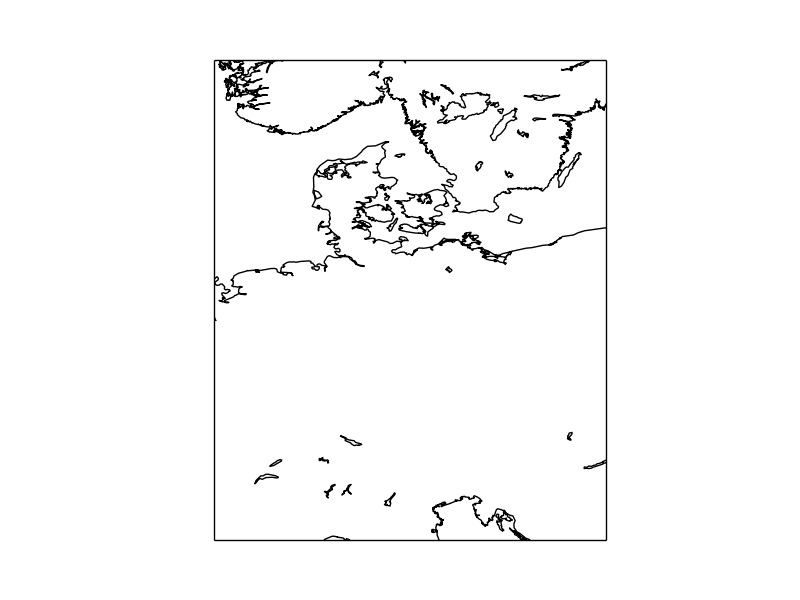
\includegraphics[scale=0.4]{/Users/student/seminar/bsp/bspcoast}\newpage 
\subsubsection*{Ländergrenzen zeichnen}
Ländergrenzen können mit der Funktion \textsf{ drawcountries(linewidth=0.5, linestyle='solid', color='k', antialiased=1, ax=None, zorder=None)} gezeichnet werden. Die Parameter sind die selben wie beim zeichnen der Küstenlinien. \\
Mit der Funktion \textsf{drawcounties(linewidth=0.1, linestyle='solid', color='k', antialiased=1, facecolor='none', ax=None, zorder=None, drawbounds=False)} können die Countiegrenzen in den USA gezeichnet werden. Mit dem Parameter \textsf{facecolor} kann eine Farbe angegeben werden mit der gefüllt werden soll.\\
Mit der Funktion \textsf{drawstates(linewidth=0.5, linestyle='solid', color='k', antialiased=1, ax=None, zorder=None)} können die Staatsgrenzen in den USA gezeichnet werden.\\
\lstinputlisting{/Users/student/seminar/bsp/bspland.py}
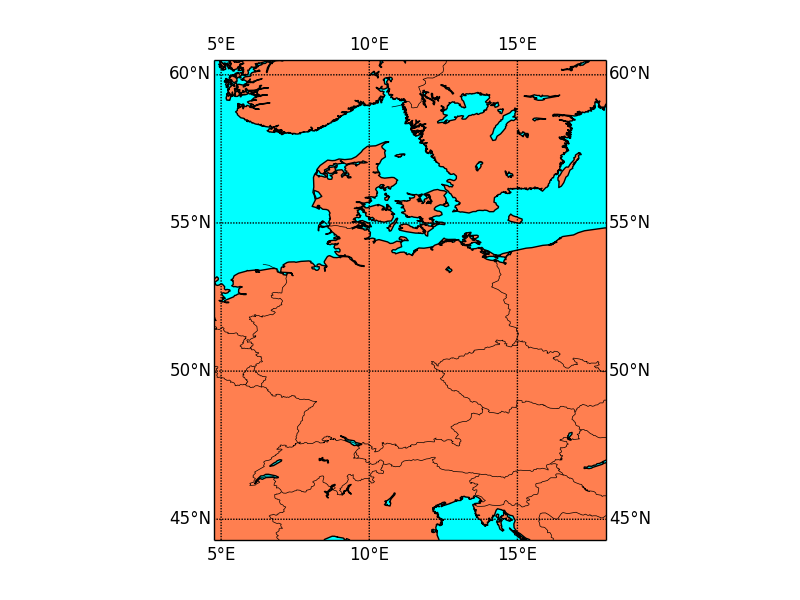
\includegraphics[scale=0.4]{/Users/student/seminar/bsp/bspland}\newpage 
 \subsubsection*{Fülle der Karte}
 Mit der Funktion \textsf{fillcontinents(color='0.8', lake\_color=None, ax=None, zorder=None, alpha=None)} kann man die Kontinente und Seen mit Farben füllen.
 Mit der Funktion \textsf{drawmapboundary(color='k', linewidth=1.0, fill\_color=None, zorder=None, ax=None)} kann man die Kartengrenze zeichnen und die Karte mit einer Farbe füllen. So kann man die Ozeane mit einer Farbe füllen, wenn man die Kontinente ebenfalls mit Farbe füllt. Sonst hat alles die gleiche Farbe.\\
 Man kann die Karte auch mit Hilfe der Funktion \textsf{drawlsmask(land\_color='0.8', ocean\_color='w', lsmask=None, lsmask\_lons=None, lsmask\_lats=None, lakes=True, resolution='l', grid=5, **kwargs)} füllen.
 Diese Funktion zeichnet ein Bild, daher kann man keine Zeichenreihenfolge angeben. Die Funktion erwartet im Parameter \textsf{lsmask} eine Matrix mit den Werten 0 für ein Ozean Pixel, 1 für ein Land Pixel und 2 für ein See Pixel. In den Parametern \textsf{lsmask\_lon} und \textsf{lsmask\_lat} erwartet die Funktion eindimensionale Arrays für die Längen- und Breitengrade der \textsf{lsmask}, sie müssen aufsteigend sortiert sein.\\
 \lstinputlisting{/Users/student/seminar/bsp/bspbase.py}
 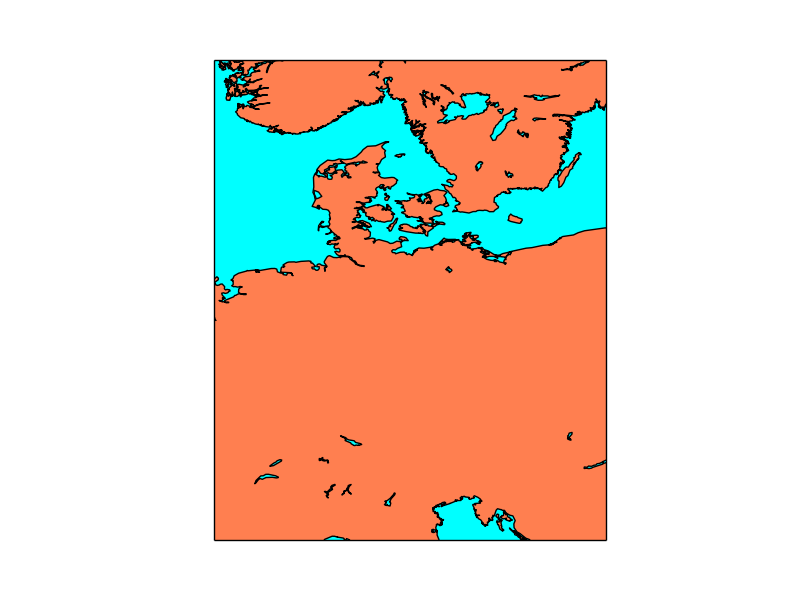
\includegraphics[scale=0.4]{/Users/student/seminar/bsp/bspbase}\newpage 
 \subsubsection*{Flüsse zeichnen}
 Die Funktion \textsf{drawrivers(linewidth=0.5, linestyle='solid', color='k', antialiased=1, ax=None, zorder=None)} ermöglicht es Flüsse zu zeichnen. Es sind allerdings nicht alle Flüsse erfasst. Die größeren sind allerdings erfasst.\\
 \lstinputlisting{/Users/student/seminar/bsp/bsprivers.py}
 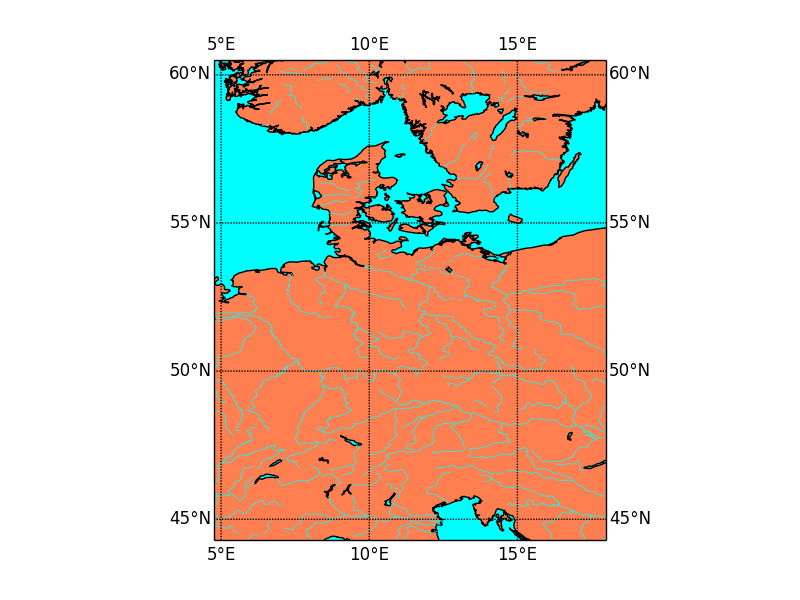
\includegraphics[scale=0.4]{/Users/student/seminar/bsp/bsprivers}\newpage 
 \subsubsection*{Längen- und Breitengrade zeichnen}
 Längen- und Breitengrade kann man einfach mit den Funktionen \textsf{drawmeridians(meridians, color='k', linewidth=1.0, zorder=None, dashes=[1, 1], labels=[0, 0, 0, 0], labelstyle=None, fmt='\%g', xoffset=None, yoffset=None, ax=None, latmax=None, **kwargs)} und \textsf{drawparallels(circles, color='k', linewidth=1.0, zorder=None, dashes=[1, 1], labels=[0, 0, 0, 0], labelstyle=None, fmt='\%g', xoffset=None, yoffset=None, ax=None, latmax=None, **kwargs)} zeichnen. Der Parameter \textsf{labels} gibt an wo die Grade beschriftet werden sollen links, rechts, oben, unten. Mit dem Parameter \textsf{labelstyle} kann man einstellen ob die Grade mit $ \pm $ oder mit E, W beziehungsweise N, S beschriftet werden sollen. Falls nichts angegeben wird, werden die Buchstaben benutzt. Dem Parameter \textsf{fmt} kann eine Funktion übergeben werden die aus dem Gradwert eine Zeichenkette macht.
 Mit dem Parameter \textsf{meridians} beziehungsweise \textsf{circles} wird eine Liste der Grade übergeben die gezeichnet werden sollen. Über den Parameter \textsf{dashes} kann man ein Pattern definieren mit dem die Grade gezeichnet werden sollen. Es werden immer abwechselnd die Anzahl an Pixeln angegeben, die gezeichnet und nicht gezeichnet werden sollen.\\
 \lstinputlisting{/Users/student/seminar/bsp/bspgrad.py}
 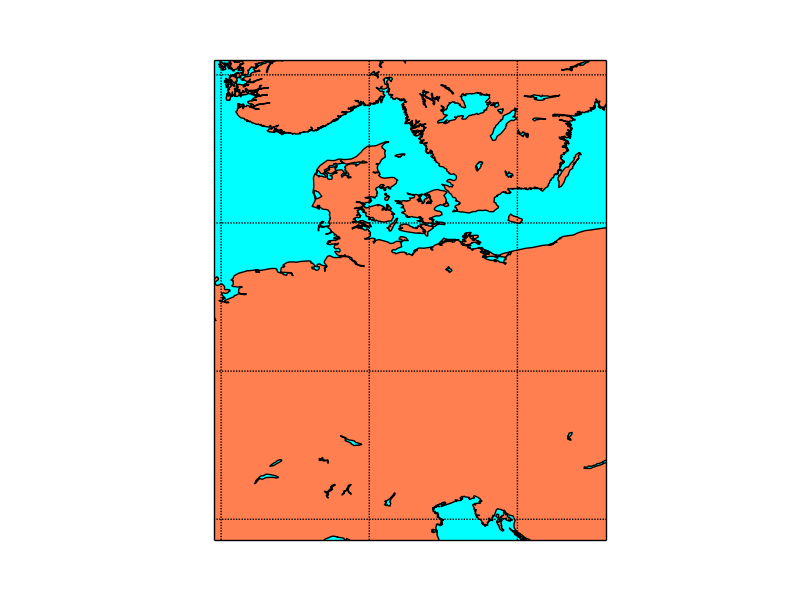
\includegraphics[scale=0.4]{/Users/student/seminar/bsp/bspgrade}
 Mit Beschriftungen:\\
  \lstinputlisting{/Users/student/seminar/bsp/bspgradlabel.py}
  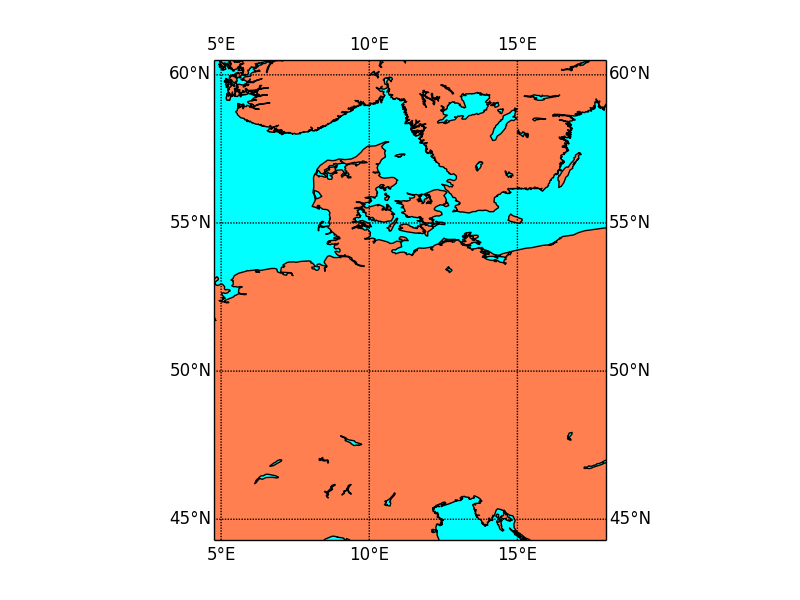
\includegraphics[scale=0.4]{/Users/student/seminar/bsp/bspgradelabel}\newpage 
 \subsubsection*{Maßstab zeichnen}
 Um einen Maßstab zu zeichnen braucht man die Funktion \textsf{drawmapscale(lon, lat, lon0, lat0, length, barstyle='simple', units='km', fontsize=9, yoffset=None, labelstyle='simple', fontcolor='k', fillcolor1='w', fillcolor2='k', ax=None, format='\%d', zorder=None)}. Diese Funktion kann nicht mit der Projektion \textsf{cyl} ausgeführt werden. Die Funktion zeichnet eine Skala an der Position \textsf{lon, lat} der Länge \textsf{length} von dem Punkt \textsf{lon0, lat0}. Die beiden Positionen sind wichtig da die Projektion längenverzerrend sein kann. Man kann den \textsf{barstyle} auf \textsf{fanzy} stellen, dann wird eine Skala gezeichnet bei der sich verschieden farbige Balken abwechseln. Wenn beim Parameter \textsf{labelstyle fancy} angegeben wird, wird über dem Balken noch der Verzerrungsfaktor und die Position \textsf{lon0, lat0} ausgegeben. Mit dem Parameter \textsf{yoffset} kann man die Höhe der Skala und die Entfernung der Beschriftung vom Balken in Metern angeben. Der Defaultwert hierfür ist 2\% der Karten Höhe.\\
 \lstinputlisting{/Users/student/seminar/bsp/bspscalar.py}
 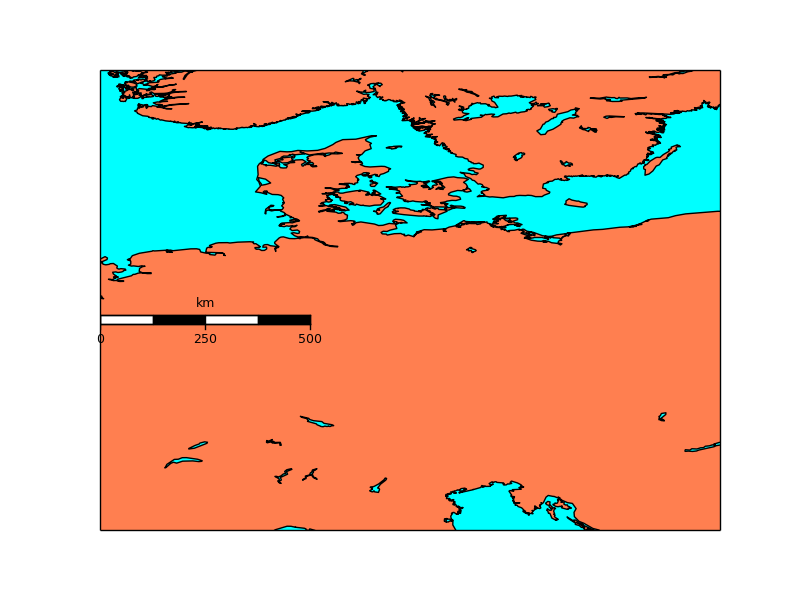
\includegraphics[scale=0.4]{/Users/student/seminar/bsp/bspscalar}\newpage 
 \subsubsection*{Relief zeichnen}
 Um eine Karte mit Relief zu zeichnen kann man die Funktionen \textsf{etopo(ax=None, scale=None, **kwargs)} oder \textsf{shadedrelief(ax=None, scale=None, **kwargs)} benutzen. Die Funktion \textsf{etopo} lädt ein ein Reliefbild von der Seite \textsf{http://www.ngdc.noaa.gov/mgg/global/global.html} als Hintergrund. Die Funktion \textsf{shadedrelief} lädt ein Reliefbild von der Seite \textsf{http://www.shadedrelief.com} als Hintergrund. Mit dem Parameter \textsf{scale} kann man einen Skalierungsfaktor angeben, da die Bilder 10800x5400 groß sind. Was eine gewisse Zeit zum laden und verarbeiten braucht und Speicherplatz verbraucht.\\
 Mit \textsf{shadedrelief()}:\\
 \lstinputlisting{/Users/student/seminar/bsp/bspshadereliev.py}
 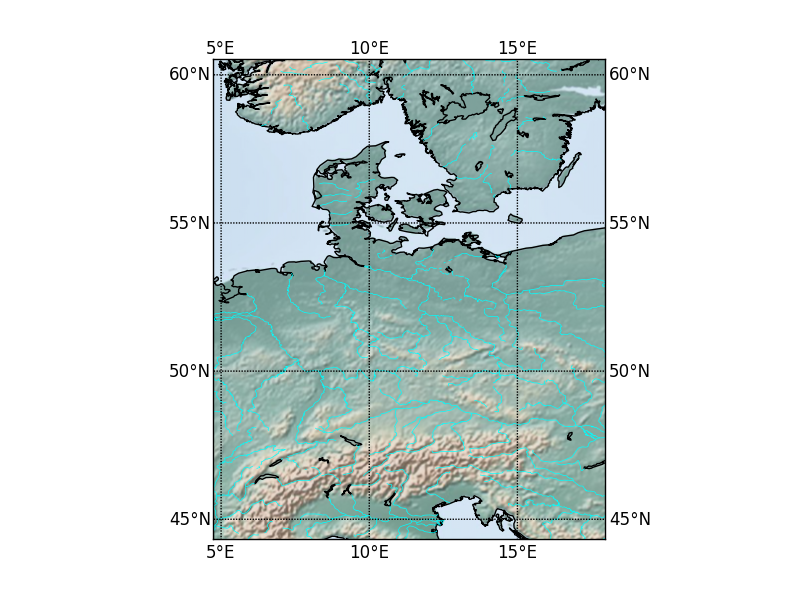
\includegraphics[scale=0.4]{/Users/student/seminar/bsp/bspshadereliev}
 Mit \textsf{etopo()}:\\
 \lstinputlisting{/Users/student/seminar/bsp/bspetopo.py}
 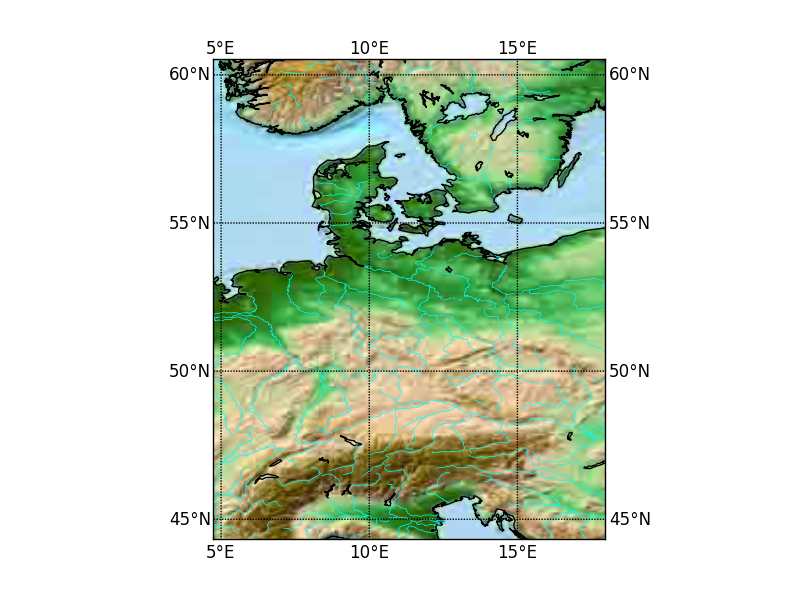
\includegraphics[scale=0.4]{/Users/student/seminar/bsp/bspetopo}